\documentclass{gapd}

\usepackage{lipsum}
\usepackage{natbib}
\usepackage{graphicx}
\usepackage{amsfonts}
\usepackage{amsmath}
\usepackage{subfigure}
\usepackage{booktabs}
\usepackage{multirow}
\usepackage{algorithm}
\usepackage[noend]{algpseudocode}
\bibliographystyle{ieeetr}

\Type{Computer Vision and Deep Learning Course Homework2}
\Title{Image Segmentation using Mean Shift Algorithm}

\Author{Letian Chen}{School of Psychological and Cognitive Sciences}

% document start
\begin{document}
\maketitle


% ==========Introduction=============
\section{Introduction}
\label{sec:Introduction}
\paragraph{}
	\lettrine{F}{}rom image classification, detection to segmentation, the task is getting harder and harder. Image classification only requires a label for the entire image, while detection requires the program to detect several objects with bounding box and label them separately. However, segmentation requires more precisely segment objects in the pixel level, i.e. to divide the pixels of image to several classes. It is clear the segmentation is much harder and has more computational burden. 

\subsection{Task}
\paragraph{}
	The task for this homework is image segmentation. As is said before, image segmentation requires the program to correctly divide image in the pixel level, labeling every pixel a class. For example, in the Fig. \ref{fig:segmentation}, the human is separated from sheep and sheep is separated from each other. 

\begin{figure*}[t]
	\centering
	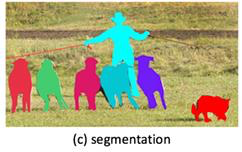
\includegraphics[width=\linewidth / 2]{graph/segmentation}
	\caption{Segmentation Demonstration}
	\label{fig:segmentation}
\end{figure*}

\subsection{Algorithm Review}
\paragraph{}
	Researchers have proposed a lot of algorithms to tackle the hard image segmentation problem. We could divide them into two categories: classic and deep-learning method. 
\paragraph{}
	The classic algorithm includes unsupervised learning and interactive learning. In unsupervised learning algorithms, the "mean shift" \cite{comaniciu2002mean} and "Graph Cut" \cite{felzenszwalb2004efficient} algorithm is the most widely accepted algorithm. Mean shift is the main algorithm in this report and we will introduce it in the Section \ref{sec:Method}. "Graph Cut", however, is to model the image as an graph and use minimal flow in graph theory to solve a minimum graph cut in the image. Interactive learning means that user could interact with the program somehow, for example, draw a rough outline for image matting and then run segmentation algorithms using the sketch as a guide. The representative algorithm in interactive learning includes "Grab Cut" \cite{rother2004grabcut} and lazy-snapping \cite{li2004lazy}. 
\paragraph{}
	As deep learning develops, deep-learning based image segmentation algorithms have been brought forward and their performance has exceeded classic methods. The representative work includes FCN \cite{long2015fully}, SegNet \cite{badrinarayanan2017segnet} and DeepLab \cite{chen2018deeplab}. As the goal of this homework is to implement a classic algorithm, we won't explain deep algorithms here. 
		
\subsection{This Report}
\paragraph{}
	In this report, we introduced the task and some classic algorithms in Section \ref{sec:Introduction}. Then, we will explain the method we use, the difficulty we face and the solution to tackle these problems in Section \ref{sec:Method}. After that, we will show our algorithm's result. Finally we will have a discussion in Section \ref{sec:Discussion}. 
	
% ==========/Introduction=============


% ==========Method=============
\section{Method}
\label{sec:Method}
		
\subsection{Mean Shift}
\label{sec:mean shift}
\paragraph{}
	Mean Shift algorithm is proposed by Comaniciu, Dorin and Meer, Peter in 2002 \cite{comaniciu2002mean}. It is a unsupervised algorithm, which means that it do not need training to find the structure of data, in this case, several clusters of pixels. The main idea of "Mean Shift" algorithm is to find several mode in the image, and points that converge to the same mode are considered as the same cluster. 
\paragraph{}
	Specifically, the algorithm contains two steps: 
	\begin{enumerate}
		\item Mode Search: In this step, we will try searching modes from several start points using mean shift. 
		\item Mode Cluster: Combine near modes according to distance measure. 
	\end{enumerate}
\paragraph{}
	Mode search is described as follows: 
	\begin{enumerate}
		\item Initialize $y_{i,0} = x_i$, $x_i$ is the i-th start point. The start point is chosen every $h_s$ row and $h_s$ column. Note that $x_i$ does not only contain location information but also the RGB value of that location. It is because mean shift should be performed on feature space, while in this task the feature space consists of location (x, y) and color (RGB). Thus, $x_i$ is a five length vector. 
		\item Find all data points that satisfy the condition that ${\| \frac{z_j - y_{i,k}}{h} \|} <= bandwidth $, in which $bandwidth$ is a free parameter to control the bandwidth of "near" definition. It is worth noting that $h$ in the denominator indicates that adjustment for different dimensions in norm operation. For example, if the feature space contains coordination and color, it is obvious that they have different scales. Therefore, $h$ is a vector to make every dimension has the same scale. 
		\item After filtering $z_j$, we need to calculate the new mean by $y_{i,k+1}=\frac{\sum_{n=1}^N{g(z_n)}}{N}$, i.e. regard the mean of all "nearby" $z_j$ as the new mean. The $g()$ function is a kernel function controlling the weight according to how far it is to the current mean when summed. 
		\item If the new mean $y_{i,k+1}$ is very similar to the previous one $|y_{i,k+1} - y_{i,k}| <= bandwidth$, it means the iteration has converged, go to step 5, otherwise, go to step 2 and iterates again. 
		\item Record the converged mean $y_{i,c}$. 
	\end{enumerate}
\paragraph{}
	Mode Cluster is described as follows: for every converged mean $m_i$ that are not deleted, iterate all mean points $m_j$ and check their distance to $m_i$. The distance definition is the same as mode search: ${\| \frac{z_j - y_{i,k}}{h} \|}$. If the distance is lower than $bandwidth$, then delete $m_j$. 
	
\begin{figure*}[ht]
	\centering
	\subfigure[Input 1]{
	\begin{minipage}[t]{0.48\columnwidth}
	\centering
	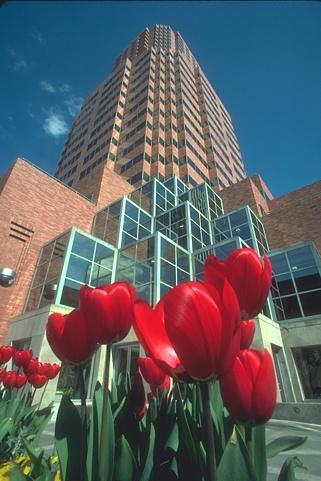
\includegraphics[width=\textwidth]{graph/input1}
	\end{minipage}
	}
	\subfigure[Input 2]{
	\begin{minipage}[t]{0.48\columnwidth}
	\centering
	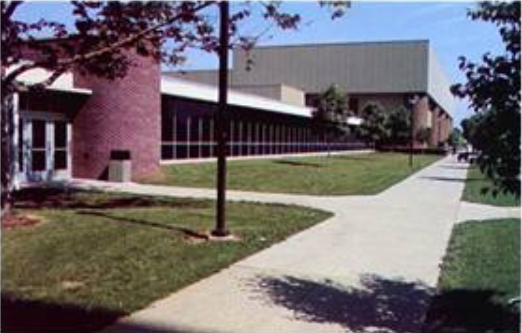
\includegraphics[width=\textwidth]{graph/input2}	
	\end{minipage}
	}
	\caption{Inputs}
	\label{fig:input}
\end{figure*}

\subsection{Implementation}
\label{sec:implementation}
\paragraph{}
	My code implementation is based on the code of \href{https://github.com/Pranshu258/meanshift}{https://github.com/Pranshu258/meanshift}. I mainly modified the calculation method of it (from serial to parallel), which will be explained in detail after. 
\paragraph{}
	To use my code, 
	\begin{enumerate}
		\item Choose one of $run\_uniform.sh$ or $run\_Gaussian.sh$. The former one's $g()$ is a uniform function while the latter one's $g()$ is a Gaussian function. 
		\item Edit the $image="XXX"$ line in either $run\_uniform.sh$ or $run\_Gaussian.sh$ to adjust the path of the original image. 
		\item Use linux style run $./run\_uniform.sh$ or $./run\_Gaussian.sh$ to run the code. 
		\item It will automatically generate 8 images using bandwidth of 10, 20, 30, 40, 50, 60, 70, 80. 
	\end{enumerate}
\paragraph{}
	The mean shift module and mean cluster module's method is the same as described in Section \ref{sec:mean shift}. The scale adjuster $h$ is $(1, 1, 1/5, 1/5, 1/5)$, in correspondence to (x, y, R, G, B) in feature space. We will see the different $bandwidth$'s impact in Section \ref{sec:Result}. The starting point stride $h_s$ we use is 40 since the image size is approximately $400 \times 400$, and in this way we could generate 100 initial start points. The way we generate starting point is: for every $40 \times 40$ pixels, we will generate a random pixel as one of starting points. 
\paragraph{}
	To generate the segmented image, we will calculate the nearest converged mode for every pixel, and then fill that pixel's RGB for them. It is worth noting that this is not the best method. The best method should be calculate the converged modes for every pixel, but the computational burden that way is quite too much and I can't just get the result of it using my laptop. Therefore, the result may not that good compared with the correct method, but it is still showing significant segmentation success. 
\subsection{Difficulty and Solution}
\paragraph{}
	Although it seems easy, I encounter many difficulties during the implementation and debugging. 
	\begin{enumerate}
		\item Parallelization: The maximum iteration times we set for each start point is 15, which means we may have to do 15 iterations for about 100 start points in the worst case. In fact, is takes me about 90s to get the result. What's worse, we will need to calculate the value for every pixel in the final segmented image drawing module, though we have done some simplification as mentioned in Section \ref{sec:implementation} to use nearest modes rather than the true converged modes. However, the program is well-parallelizable. We could easily use separate CPU core to do iterations for each 100 start points. We could also easily calculate the value for every pixel separately on separate CPU cores. After transforming the serial program into a parallel one, the mode search time decreases from 90s to 10s on a 12-core CPU. The drawing part's time decreases from I-don't-know to 70s. Since I want to do the comparison in different bandwidth, the decreased calculation time is really essential. 
		\item Choose of image: because of the difficulty of the hard, choose of image is very important if you want to see good results. As a matter of fact, mean shift is just an unsupervised algorithm, which means that the data need to demonstrate a clear pattern for the algorithm to find because the algorithm does not know the exact answer. After trying, the rule of thumb I think is to choose images that has clear color separation is a better choice since we only use location and color in our feature space. Fig. \ref{fig:segmentation} is a good example since human, sheep and background's color are all clearly different. If the difference if mainly on texture, we may use a convolution filter to firstly get texture features and add them in the feature space. 
		\item Bandwidth: bandwidth strongly influence the performance of the algorithm. In fact, larger bandwidth will cause unrelated modes to be combined, while smaller bandwidth will cause too much modes to have a good segmentation results. Thus, we tried different bandwidth in two images to see how bandwidth influence the segmentation result and what's the best bandwidth generally. 
	\end{enumerate}
	

% ==========/Method=============

% ==========Result=============
\section{Result}
\label{sec:Result}
\begin{figure*}[ht]
	\centering
	\subfigure[Uniform]{
	\begin{minipage}[t]{0.8\columnwidth}
	\centering
	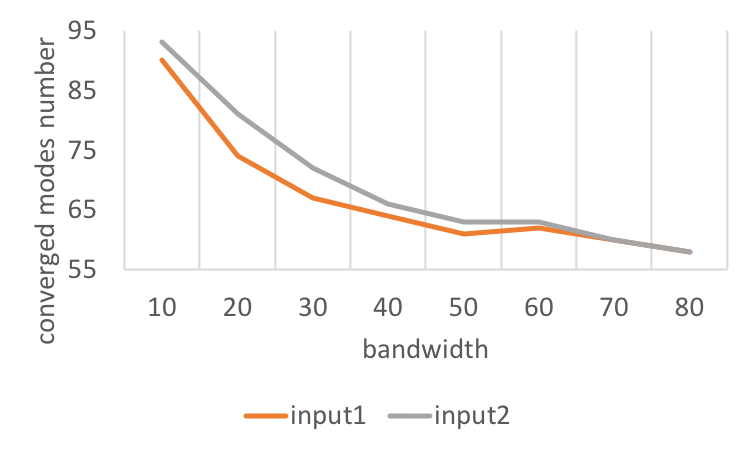
\includegraphics[width=\textwidth]{graph/input1_bandwidth}
	\end{minipage}
	}
	\subfigure[Gaussian]{
	\begin{minipage}[t]{0.8\columnwidth}
	\centering
	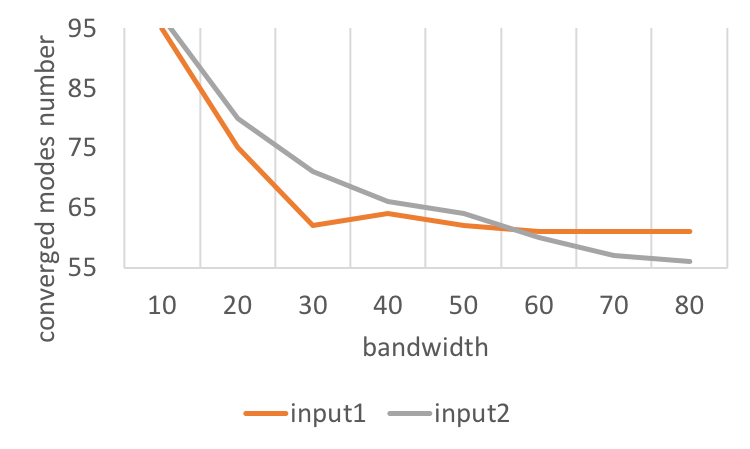
\includegraphics[width=\textwidth]{graph/input2_bandwidth}
	\end{minipage}
	}
	\caption{Converged modes number in different Bandwidths}
	\label{fig:bandwidth}
\end{figure*}
\begin{figure*}[ht]
	\centering
	\subfigure[Bandwidth=10]{
	\begin{minipage}[t]{0.6\columnwidth}
	\centering
	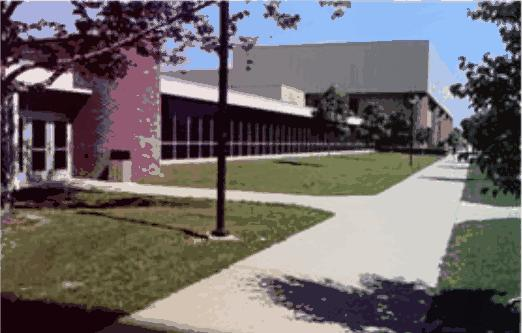
\includegraphics[width=\textwidth]{graph/gaussian_output_input2_10}
	\end{minipage}
	}
	\subfigure[Bandwidth=30]{
	\begin{minipage}[t]{0.6\columnwidth}
	\centering
	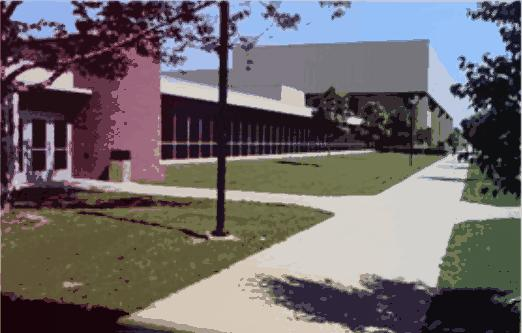
\includegraphics[width=\textwidth]{graph/gaussian_output_input2_30}
	\end{minipage}
	}
	\caption{Segmentation Result for Input 2 in Different Bandwidth}
	\label{fig:different_bandwidth_input_2}
\end{figure*}	
\paragraph{}
	\lettrine{W}{}e use two images to demonstrate the segmentation result. They are shown in Fig. \ref{fig:input}. We could see that the first image is harder than the second one because the second one's color separation is obvious while the first one's color on flowers and leaves is strongly influenced by light. 

\paragraph{}
	Firstly, we'd like to see how bandwidth will influence the segmentation result. Different converged modes numbers in different bandwidths is shown in Fig. \ref{fig:bandwidth}. Fig. \ref{fig:bandwidth}(a) uses uniform $g()$ in calculating the new mass mean, while Fig. \ref{fig:bandwidth}(b) uses Gaussian $g()$. We could see that in uniform $g()$, the bandwidth of 40 seems to be a turning point that after bigger bandwidth will result in no change of converged modes number. Nonetheless, in the Gaussian $g()$, the turning point is at the bandwidth of 30. Therefore, we regard the 40 is the best bandwidth for uniform $g()$ while 30 is the best bandwidth for Gaussian $g()$. We could also see the effect of different bandwidth in Fig \ref{fig:different_bandwidth_input_2}. 
	
\begin{figure*}[ht]
	\centering
	\subfigure[Original]{
	\begin{minipage}[t]{0.5\columnwidth}
	\centering
	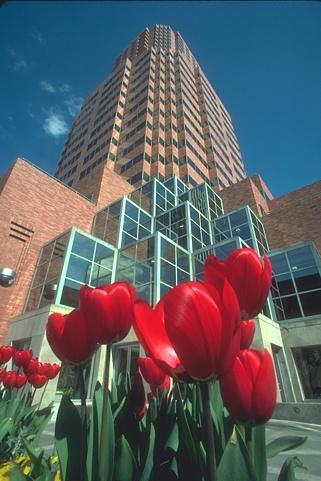
\includegraphics[width=\textwidth]{graph/input1}
	\end{minipage}
	}
	\subfigure[Uniform]{
	\begin{minipage}[t]{0.5\columnwidth}
	\centering
	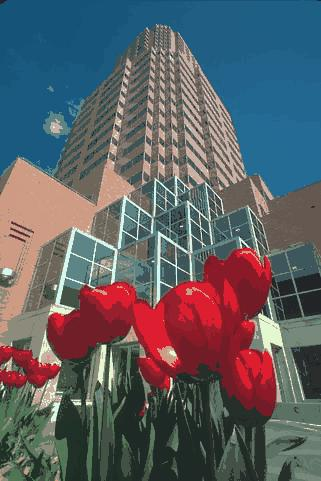
\includegraphics[width=\textwidth]{graph/uniform_output_input1_40}
	\end{minipage}
	}
	\subfigure[Gaussian]{
	\begin{minipage}[t]{0.5\columnwidth}
	\centering
	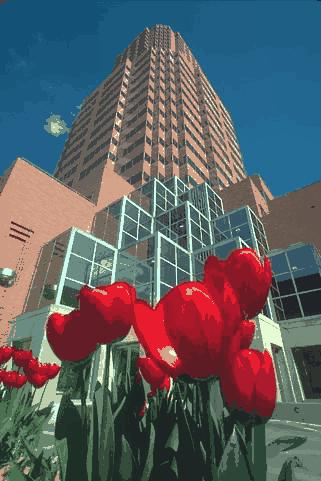
\includegraphics[width=\textwidth]{graph/gaussian_output_input1_30}
	\end{minipage}
	}
	\caption{Segmentation Result for Input 1}
	\label{fig:input1_result}
\end{figure*}
\begin{figure*}[ht]
	\centering
	\subfigure[Original]{
	\begin{minipage}[t]{0.6\columnwidth}
	\centering
	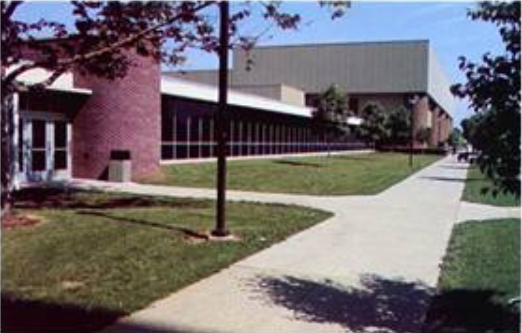
\includegraphics[width=\textwidth]{graph/input2}
	\end{minipage}
	}
	\subfigure[Uniform]{
	\begin{minipage}[t]{0.6\columnwidth}
	\centering
	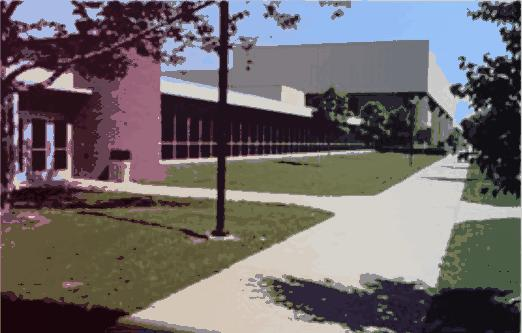
\includegraphics[width=\textwidth]{graph/uniform_output_input2_40}
	\end{minipage}
	}
	\subfigure[Gaussian]{
	\begin{minipage}[t]{0.6\columnwidth}
	\centering
	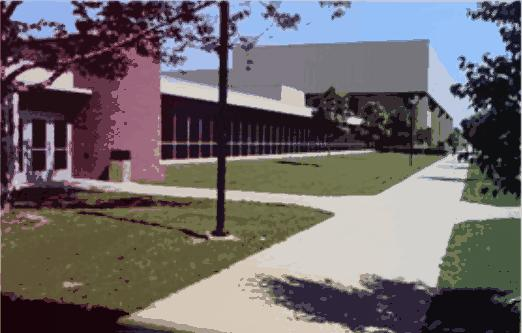
\includegraphics[width=\textwidth]{graph/gaussian_output_input2_30}
	\end{minipage}
	}
	\caption{Segmentation Result for Input 2}
	\label{fig:input2_result}
\end{figure*}
\paragraph{}
	We demonstrate our segmentation result for input1 in Fig. \ref{fig:input1_result}. It is obvious that both uniform and gaussian $g()$ successfully segment the image into 60+ classes. But as we said before, this image's color is highly influenced by light, which makes that flowers and leaves being separated into several classes. 
\paragraph{}
	In the segmentation result for input 2 (See Fig. \ref{fig:input2_result}), we could clearly see the kermesinus cylindrical building is successfully divided into three classes, from most bright to most dim. The grass is almost separated into the same class. Therefore, in order to make mean shift algorithm do its job better, we should pick images that different objects have different colors. 
\paragraph{}
	We could also see that gaussian segmentation is a little bit better than uniform segmentation, since it seems more smooth in both input1 and input2 figures. 
% ==========/Result=============


% ==========Discuss and conclusion=============
\section{Discussion}
\label{sec:Discussion}
\paragraph{}
\lettrine{I}{}n this project, we learned the task of image segmentation, the idea of mean shift and implement our own version of mean shift algorithm. The algorithm works well in two representative images, though the result seems better in the second image because it is relatively easy because of the obvious color separation in different segments. Also, we demonstrate the difference when using different bandwidths in the separation. We conclude that for uniform mean calculation, bandwidth of 40 is better while for Gaussian mean calculation, bandwidth of 30 is better. We also parallelize the program to make it at least 10x faster than the original implementation. 
\paragraph{} 
	However, our implementation still have several problems. For example, as said in Section \ref{sec:implementation}, we do not use every pixel's true convergence point to be its class, but use the nearest modes as its class to decrease the computational burden. In fact, the calculation could be further parallelized to make exact calculation possible. Moreover, we could also transform many calculation into matrix calculation to put them run on GPU to gain an even faster performance. Besides, mean shift is still only an unsupervised algorithm. Hence, the segmentation result is not very good compared to interactive algorithms or trained deep-learning algorithms. To make it better, the choose of feature space is essential. 
			
% ==========/Discuss and conclusion=============

\section{Reference}
\bibliography{reference}

\end{document}
